\documentclass[10pt,twocolumn,letterpaper]{article}

\usepackage{iccv}
\usepackage{times}
\usepackage{epsfig}
\usepackage{graphicx}
\usepackage{amsmath}
\usepackage{amssymb}

% Include other packages here, before hyperref.

% If you comment hyperref and then uncomment it, you should delete
% egpaper.aux before re-running latex.  (Or just hit 'q' on the first latex
% run, let it finish, and you should be clear).
\usepackage[pagebackref=true,breaklinks=true,letterpaper=true,colorlinks,bookmarks=false]{hyperref}

 \iccvfinalcopy % *** Uncomment this line for the final submission

% Pages are numbered in submission mode, and unnumbered in camera-ready
\ificcvfinal\pagestyle{empty}\fi

\begin{document}

%%%%%%%%% TITLE
\title{CAP 5516 Medical Image Computing Spring 2022 Assignment 1: Pneumonia Classification from Chest X-Ray}

\author{Kyle Beggs\\
Department of Mechanical and Aerospace Engineering\\ 
University of Central Florida\\
{\tt\small kbeggs07@knights.ucf.edu}}

\maketitle
% Remove page # from the first page of camera-ready.
\ificcvfinal\thispagestyle{empty}\fi


%%%%%%%%%%%%%%%%%%%%%%%%%%%%%%%%%%%%%%%%%%%%%%%%%%%%%%%%%%%%%%%%%%%%%%%%%%%%%%%
\begin{abstract}
    DOnt forget to fill this out!
\end{abstract}


%%%%%%%%%%%%%%%%%%%%%%%%%%%%%%%%%%%%%%%%%%%%%%%%%%%%%%%%%%%%%%%%%%%%%%%%%%%%%%%
\section{Problem Definition}

The most common diagnostic for patients that are suspected to have pneumonia is a chest x-ray. After the x-ray is taken, a radiologist looks at the image and determines if the patient is positive or negative for pneumonia. Automating this process would save much time for physicians on a routine task. The goal of this project is to build a deep learning model to detect pneumonia in pediatric chest x-rays.


%%%%%%%%%%%%%%%%%%%%%%%%%%%%%%%%%%%%%%%%%%%%%%%%%%%%%%%%%%%%%%%%%%%%%%%%%%%%%%%
\section{Methods}
Due to limited compute resource, the ResNet18 network (Figure \ref{fig:fig1}) is chosen to perform the classification task as it has few learnable parameters compared to top performing networks, yet only suffers little in performance. The network is trained both with random initialization of weights and using pretrained weights found from training the network on ImageNet.

\begin{figure}[h]
\begin{center}
   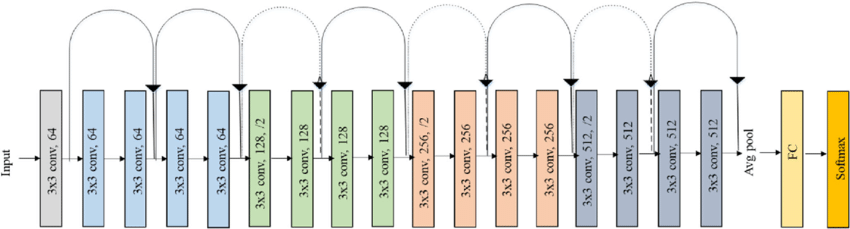
\includegraphics[width=0.95\linewidth]{images/Original-ResNet-18-Architecture.png}
\end{center}
   \caption{ResNet18 Architecture.}
\label{fig:fig1}
\end{figure}

The dataset is taken from Kaggle (https://www.kaggle.com/paultimothymooney/chest-xray-pneumonia) containing 5856 images in total. There are 5216 in the training set, 16 in the validation set, and 624 in the test set. There are only 2 classes - `normal' which is pneumonia negative and `pneumonia' which is positive for the condition. the classes are imbalanced, as the `normal' class makes up 25.7\% of the training set while the `pneumonia' class makes up the rest at 74.3\%. Class imbalance is addressed through weighting the loss function according to the inverse of the percent of the datset that class represents. Data augmentation is performed by randomly flipping about the x and y axis, both with 50\% probability as well as randomly zooming between a range of 0.9-1.1 with a 50\% probablity. An example of the original image and its transform, as well as their histograms are shown in Figure \ref{fig:fig2}.

\begin{figure}[h]
\begin{center}
   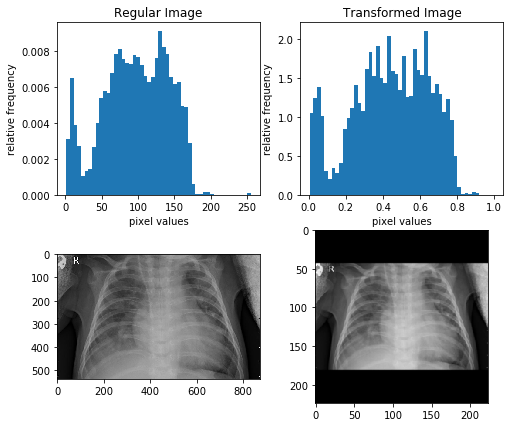
\includegraphics[width=0.95\linewidth]{images/hist_and_transform1.png}
\end{center}
   \caption{Histogram and display of original image (left) and transformed image (right).}
\label{fig:fig2}
\end{figure}

The images are preprocessed by padding with 0's such that they are square as the aspect ratios of the images in the datasets are not constant. Then the image is resized to 224x224 for computational efficiency reasons, as well as this was the original image size ResNet was used for. The image is ensured to be 1 channel (greyscale) and lastly the image is scaled according to its intensity.

The batch size is set to 8 due to GPU memory limitations. The learning rate is initially set to 0.00005 and is set to decay according to a reduction of 30\% of the current value every 10 epochs. The model is trained for 100 epochs every time with no early stopping. The weights are saved from the last epoch of each run for evaluation of model performance using the test set.

%%%%%%%%%%%%%%%%%%%%%%%%%%%%%%%%%%%%%%%%%%%%%%%%%%%%%%%%%%%%%%%%%%%%%%%%%%%%%%%
\section{Results}

The model is incrementally trained - meaning we begin with a most basic model and keep adding complexities that in theory should increase the performance of the model. Four models are completed, each including everything of the model before:
\begin{enumerate}
   \item Basic model with random weight initialization.
   \item Data augmentation.
   \item Pretrained with ImageNet.
   \item Class imbalance addressed through loss weighting.
\end{enumerate}

A bonus is also trained where the model is pretrained, balanced, with \emph{no augmentation}. The training and validation loss is shown in Figures \ref{fig:fig3} and \ref{fig:fig4} and the validation accuracy is shown in Figure \ref{fig:fig5}.

\begin{figure}[h]
   \begin{center}
      \textbf{Training Loss}\par\medskip
      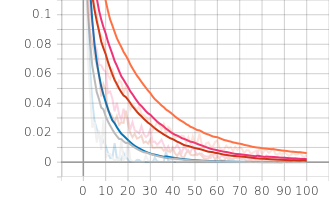
\includegraphics[width=0.95\linewidth]{images/loss-training.png}
   \end{center}
   \caption{Training loss curves for training set. Curve colors: blue is random initialization with no augmentation, orange is random initialization with augmentation, red is pretrained with augmentation, pink is pretrained with augmentation that is balanced, and grey is pretrained with balancing and no augmentation.}
\label{fig:fig3}
\end{figure}

\begin{figure}[h]
   \begin{center}
      \textbf{Validation Loss}\par\medskip
      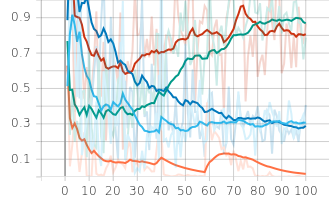
\includegraphics[width=0.95\linewidth]{images/loss-val.png}
   \end{center}
   \caption{Validation loss curves for training set. Curve colors: red is random initialization with no augmentation, blue is random initialization with augmentation, light blue is pretrained with augmentation, green is pretrained with augmentation that is balanced, and orange is pretrained with balancing and no augmentation.}
\label{fig:fig4}
\end{figure}

\begin{figure}[h]
   \begin{center}
      \textbf{Validation Accuracy}\par\medskip
      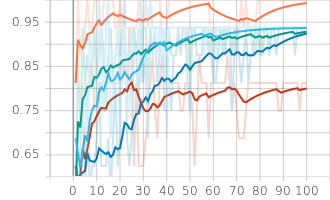
\includegraphics[width=0.95\linewidth]{images/accuracy-val.png}
   \end{center}
   \caption{Accuracy curves for validation set. Curve colors: red is random initialization with no augmentation, blue is random initialization with augmentation, light blue is pretrained with augmentation, green is pretrained with augmentation that is balanced, and orange is pretrained with balancing and no augmentation.}
\label{fig:fig5}
\end{figure}

The test set is evaluated as the results are shown in Tables \ref{table:table1} and \ref{table:table2}.

\begin{table}[h]
   \begin{center}
      \begin{tabular}{l l l}
         Model Settings &
         \multicolumn{1}{p{5em}}{\centering Accuracy  \\ (Overall)} &
         F1 \\ 
         \hline
         Random & 0.8685 & 0.7297 \\
         Random w/ Aug. & 0.8741 & 0.7602 \\
         Pre. w/ Aug. & 0.8869 & 0.7752 \\
         Pre. w/ Aug. \& Bal. & 0.8866 & 0.7853 \\
         Pre. \& Bal. & 0.8974 & 0.8145 \\
      \end{tabular}
   \end{center}
\caption{Results of test set showing overall accuracy for both classes and F1 score. `Pre.' is for pretrained with ImageNet, `Aug.' is for data augmentation, and `Bal.' is when class imbalance was addressed.}
\label{table:table1}
\end{table}


\begin{table}[h]
   \begin{center}
       \begin{tabular}{l l l l l}
         Model Settings &
         \multicolumn{1}{p{6em}}{\centering Accuracy  \\ (Pneumonia)} &
         \multicolumn{1}{p{6em}}{\centering Accuracy  \\ (Normal)} \\
         \hline
         Random & 0.7466 & 0.9903 \\
         Random w/ Aug. & 0.7653 & 0.9829 \\
         Pre. w/ Aug. & 0.7738 & 1.0000 \\
         Pre. w/ Aug. \& Bal. & 0.7811 & 0.9921 \\
         Pre. \& Bal. & 0.8021 & 0.9928 \\
      \end{tabular}
   \end{center}
   \caption{Results of test set showing accuracy for each class. `Pre.' is for pretrained with ImageNet, `Aug.' is for data augmentation, and `Bal.' is when class imbalance was addressed.}
   \label{table:table2}
\end{table}


%%%%%%%%%%%%%%%%%%%%%%%%%%%%%%%%%%%%%%%%%%%%%%%%%%%%%%%%%%%%%%%%%%%%%%%%%%%%%%%
\section{Discussion}

AS shown in Tables \ref{table:table1} and \ref{table:table2}, the best performing model (according the F1 score) was pretrained on ImageNet, and class balanced. Conventional wisdom expects these settings with the addition of data augmentation to be the best, however it performs second best implying augmentation to be detrimental to the performance of the model. There is suspicion that augmentation was too aggressive as it included flipping on both axis and zooming. After re-examination of the original images, they are all oriented correctly, so flipping upon axis does not make sense. Slight zoom in or out is evident throughout the dataset. It is suggested to slightly rotate the images as well. It is not clear why misclassifications happen when looking at images only (shown in Figure \ref{fig:fig6}) and the use of TorchCAM is suggested.

\begin{figure}[h]
   \begin{center}
      \textbf{Misclassified Images.}\par\medskip
      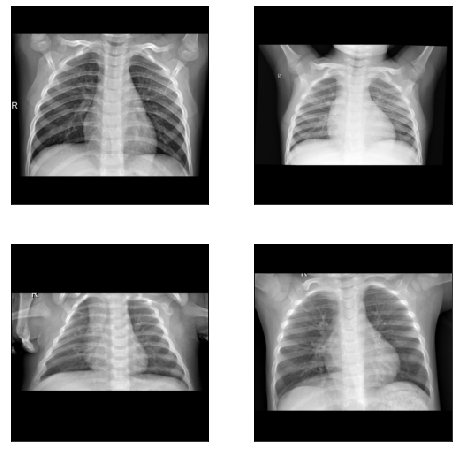
\includegraphics[width=0.95\linewidth]{images/misclassfied.png}
   \end{center}
   \caption{Transformed images that are misclassified by the best-performing model.}
\label{fig:fig6}
\end{figure}

The code can be found on GitHub at \href{https://github.com/kylebeggs/Pediatric-Pneumonia-Classification-from-XRay}{kylebeggs/Pediatric-Pneumonia-Classification-from-XRay}.

\end{document}
